\begin{problem}{Missing}{standard input}{standard output}{1 second}{256 megabytes}

$F$or a long time, $Mazen$ did not meet his friend $Mahmoud$, so he decided to visit him at the same time that $Mahmoud$ decided to visit $Mazen$.

$Mazen$ and $Mahmoud$ are living in square grid consisting of $n \times n$ with rows and columns numbered from $1$ to $n$, $Mazen$ is living in cell $(1,1)$ and $Mahmoud$ is living in cell $(n,n)$.

$So$ in each move:
\begin{itemize}
  \item $Mazen$ can go $Down$ and then $Right$.
  \item $Mahmoud$ can go $Up$ and then $Left$.
\end{itemize}

$You$ need to determine whether they will meet each other in any cell.

\InputFile
The first line contains $t$ $(1 \le t \le 1000)$ -- $t$ donates numbers of test cases.

Each line contains $n$ $(2 \le n \le 10^3)$ -- $n$ is the dimension of the grid.

\OutputFile
In each test case if $Mazen$ will meet $Mahmoud$ print \textbf{``YES``} or he will not find him print \textbf{``NO``}.

The strings \bf{``yEs``}, \bf{``yes``}, \bf{``Yes``} and \bf{``YES``} will be recognized as a positive answer.

\Example

\begin{example}
\exmpfile{example.01}{example.01.a}%
\end{example}

\Note
For $N$ = 5:

1- Initially $Mazen$ and $Mahmoud$ place.
\begin{center}
  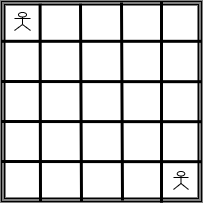
\includegraphics[scale=1.5]{Initialyf.drawio.png} \\
  \small{}
\end{center}

2- After $first$ move$:$
\begin{center}
  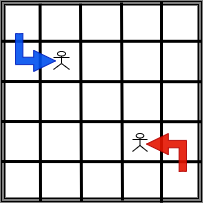
\includegraphics[scale=1.5]{First_Move.drawio.png} \\
  \small{}
\end{center}

3- Afer $Second$ move $Mazen$ and $Mahmoud$ will be at the same cell:
\begin{center}
  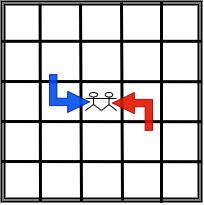
\includegraphics[scale=1.5]{Second_Move.drawio.png} \\
  \small{}
\end{center}

\end{problem}

